% Drawing 154/02-11 -- folder 154, batch 02, archive page 37 (PDF page 38).
% Transcription: figure à gauche du texte : un disque au bord vert (clair et foncé) traversé de cordes orange, cinq régions voisines du bord hachurées en jaune, deux petits segments bleus en haut et en bas du bord
% Kind: chord system in a disk, regions by the rim coloured. Method 2 (schematic redraw from the facsimile). Status: partial.
% Notes: Left of the text: a disk with a green rim (dark green on the left, light green elsewhere) crossed by orange chords; five regions next to the rim hatched in yellow-orange; two short blue segments at the top and the bottom of the rim. Read from the page view; chords schematic, the five regions placed approximately.
% Coordinates: 1 unit = 1 mm = 1/100 of the crop width (bbox in page fractions: [0.134, 0.319, 0.279, 0.422]).
% Redrawn by Claude (claude-opus-5-5), issue #73, 2026-11-07; not checked by a human; not compiled (no TeX in the session).
% Rights: reproduces part of the work -- behind RENDER_TRANSCRIPTS, never published by itself.
\documentclass[tikz,border=3pt]{standalone}
\usepackage{amsmath,amssymb}
\usetikzlibrary{patterns,arrows.meta}
\tikzset{Or/.style={orange!90!black}, Ye/.style={yellow!80!orange}, Lg/.style={green!60!black!70}, Dg/.style={green!45!black}, Br/.style={brown!80!black}, Rd/.style={red!85!black}, Bl/.style={blue!70!black}, Gy/.style={black!40}, pencil/.style={black!45}, struck/.style={black!35}, mark/.style={circle,draw,inner sep=1.3pt}, pt/.style={circle,fill,inner sep=0.9pt}, opt/.style={circle,draw,fill=white,inner sep=1.1pt}}
\begin{document}
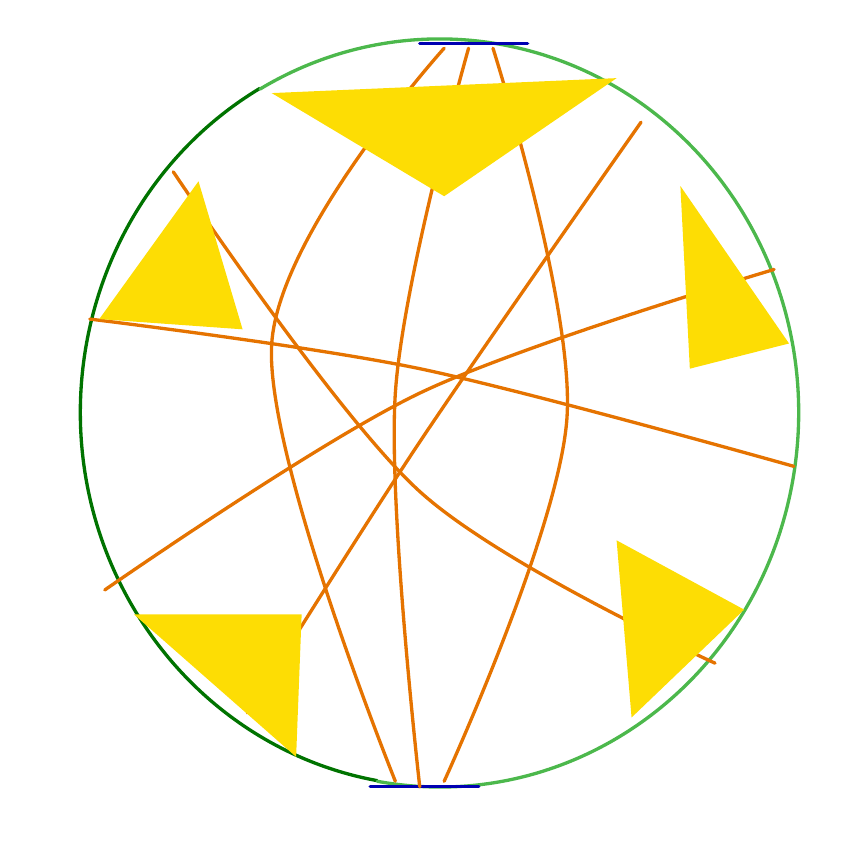
\begin{tikzpicture}[x=1mm,y=1mm,line cap=round,line join=round,font=\scriptsize]
\draw[Dg,very thick] (26.6,-8.2) arc[start angle=120, end angle=260, x radius=45.6, y radius=47.5];
\draw[Lg,very thick] (41.5,-96.2) arc[start angle=-100, end angle=120, x radius=45.6, y radius=47.5];
\draw[Bl,very thick] (46.9,-2.5) -- (60.6,-2.5);
\draw[Bl,very thick] (40.6,-96.9) -- (54.4,-96.9);
\draw[Or,very thick] plot[smooth, tension=0.55] coordinates {(53.1,-3.1) (43.8,-46.9) (46.9,-96.9)};
\draw[Or,very thick] plot[smooth, tension=0.55] coordinates {(56.2,-3.1) (65.6,-50) (50,-96.2)};
\draw[Or,very thick] plot[smooth, tension=0.55] coordinates {(50,-3.1) (28.1,-40.6) (43.8,-96.2)};
\draw[Or,very thick] plot[smooth, tension=0.55] coordinates {(6.9,-71.9) (46.9,-46.9) (91.9,-31.2)};
\draw[Or,very thick] plot[smooth, tension=0.55] coordinates {(5,-37.5) (46.9,-43.8) (94.4,-56.2)};
\draw[Or,very thick] plot[smooth, tension=0.55] coordinates {(15.6,-18.8) (46.9,-59.4) (84.4,-81.2)};
\draw[Or,very thick] plot[smooth, tension=0.55] coordinates {(75,-12.5) (46.9,-53.1) (25,-87.5)};
\fill[pattern=north east lines,Ye] (28.1,-8.8) -- (71.9,-6.9) -- (50,-21.9) -- cycle;
\fill[pattern=north east lines,Ye] (80,-20.6) -- (93.8,-40.6) -- (81.2,-43.8) -- cycle;
\fill[pattern=north east lines,Ye] (10.6,-75) -- (31.2,-93.1) -- (31.9,-75) -- cycle;
\fill[pattern=north east lines,Ye] (71.9,-65.6) -- (88.1,-74.4) -- (73.8,-88.1) -- cycle;
\fill[pattern=north east lines,Ye] (6.2,-37.5) -- (18.8,-20) -- (24.4,-38.8) -- cycle;
\end{tikzpicture}
\end{document}
